% start of file `cv_german.tex', based on `template_en.tex` 
% by Xavier Danaux (xdanaux@gmail.com).
% This work may be distributed and/or modified under the
% conditions of the LaTeX Project Public License version 1.3c,
% available at http://www.latex-project.org/lppl/.
% 
% Thomas Quaritsch <t.quaritsch@student.tugraz.at>

\documentclass[11pt,a4paper]{moderncv}

% \usepackage[german]{babel}
\usepackage[english]{babel}
\usepackage[utf8]{inputenc}
\usepackage{multicol}
\moderncvtheme[blue]{casual}
\usepackage{moderncv-additions}

% adjust the page margins
\usepackage[scale=0.8]{geometry}
\setlength{\hintscolumnwidth}{3cm}

% if you want to change the width of the column with the dates
% \AtBeginDocument{\setlength{\maketitlenamewidth}{6cm}}
% only for the classic theme, if you want to change the width 
% of your name placeholder (to leave more space for your address details

\AtBeginDocument{\recomputelengths}
% required when changes are made to page layout lengths

% personal data
\firstname{Philipp}
\familyname{Hacker}
\address{Karl-Liebknecht-Ring 13}{17489 Greifswald}
\mobile{+49 152 052 77 686}
\email{rayleighsjeans@gmail.com}
\photo[64pt]{picture}

% \title{Resumé title (optional)}
% \phone{phone (optional)}
% \fax{fax (optional)}
% \extrainfo{additional information (optional)}

% '64pt' is the height the picture must be resized 
% to and 'picture' is the name of the picture file
% \quote{``Das ist ein toller Frusterspruch\\%
%					von Friede Frusterfrau.'' -- Friede Frusterfrau}

% \nopagenumbers{}
% uncomment to suppress automatic page numbering for CVs
% longer than one page

\newcommand{\sign}[1]{%
  \begin{tabular}[t]{@{}l@{}}
  \makebox[1.5in]{\dotfill}\\
  \strut\emph{#1}\strut%
  \end{tabular}%
}

%----------------------------------------------------------------------------------
%            content
%----------------------------------------------------------------------------------
\begin{document}

	% color redefinitions must be after \begin{document}!
	\definecolor{firstnamecolor}{RGB}{125,85,85}
	\definecolor{familynamecolor}{RGB}{138,74,57}
	\definecolor{quotecolor}{RGB}{125,85,85}
	\definecolor{addresscolor}{RGB}{125,85,85}
	\definecolor{sectionrectanglecolor}{RGB}{138,74,57}
	\definecolor{sectiontitlecolor}{RGB}{138,74,57}
	\definecolor{subsectioncolor}{RGB}{125,85,85}
	\definecolor{footersymbolcolor}{RGB}{125,85,85}	
	
	\makeatletter
	\pagestyle{empty}
	\chapter*{Application}{~Form}
	
	\vspace*{3.5cm}
	\begin{minipage}{\textwidth}
		\vspace*{3mm}
		\familynamestyle{\@firstname}~\firstnamestyle{\@familyname} 	
			\hspace*{5mm}%
			{{\color{firstnamecolor}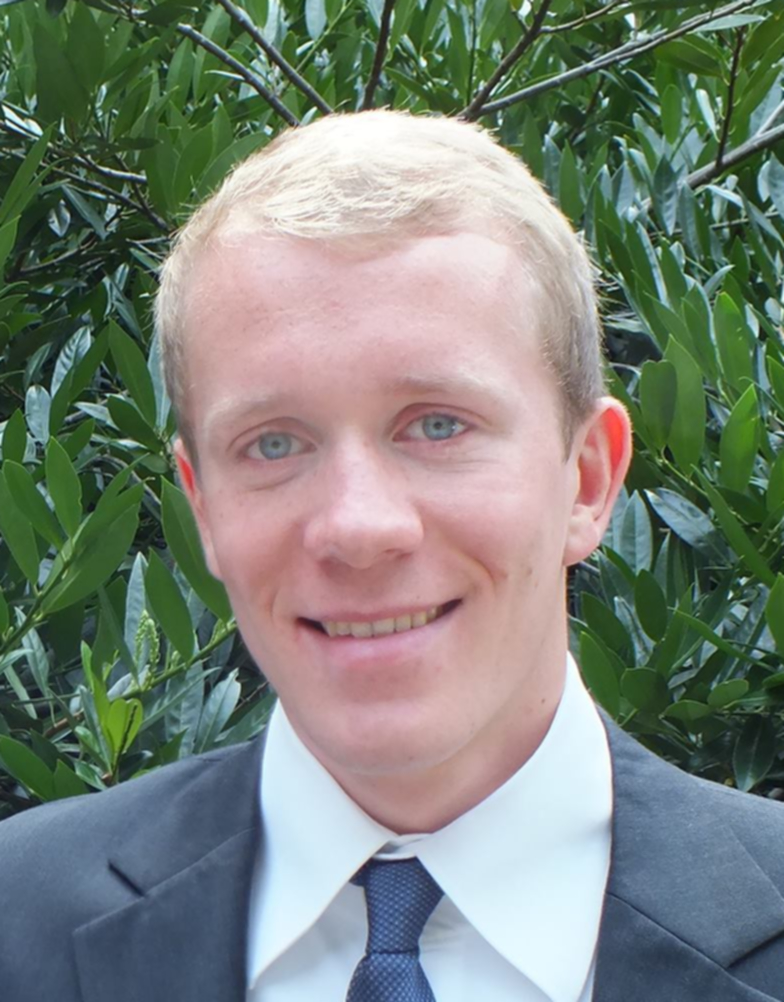
\includegraphics[width=96pt]{figures/fig/12.jpg}}}\\[0.3cm]
			\@addressstreet\\[0.0cm]%
			\@addresscity\\[0.3cm]%
			\mobilesymbol~\@mobile\\[0.3cm]%
			\emailsymbol~\@email%
	\end{minipage}
	\begin{minipage}{70pt}
	\end{minipage}
	\vfill
	\begin{minipage}{1.0\textwidth}
		\section{Contents}
		\tableofcontents
	\end{minipage}
	
	%---------------------------------------------------------------%
	%            letter 																						%
	%---------------------------------------------------------------%
	\newpage
	\makeatletter
	\chapter{Application}{~Letter}

	\vspace*{1.0cm}
	\begin{minipage}{0.6\textwidth}
		\begin{flushleft}
			Referat Z.3 - Personal\\[0.2cm]
			{\bfseries{\color{firstnamecolor}%
				Bundesanstalt für Materialforschung und -prüfung%
			}}\\[0.2cm]
			Unter den Eichen 87\\
			12205 Berlin\\
			Germany\\
			www.bam.de\\
		\end{flushleft}
	\end{minipage}
	\hfill
	\begin{minipage}{0.3\textwidth}
		\begin{flushright}
			\vspace*{1.3cm}
			Karl-Liebknecht-Ring 13\\
			17489 Greifswald\\[1.0cm]
			\today
		\end{flushright}
	\end{minipage}
	
	\vspace*{1.0cm}
	{\bfseries \color{familynamecolor}%
		Application for the Ph.D.-Position\\
		reference number 169/17-8.5
	}\\[0.75cm]
%
	Dear Mrs.\ or Mr.,\\[0.5cm]
%	
	with this form I would like to submit my initial application for the Ph.D. position referenced under the number 169/17-8.5 at the Bundesanstalt für Materialforschung und -prüfung in Berlin-Steglitz.\\[0.3cm]
%
		I am currently working on my Master thesis under the supervision of Prof. Dr. Ralf Schneider at the Institute of Physics of the Ernst-Moritz-Arndt University in Greifswald. On September the 11th I will submit this work. My Master of Science degree will presumably be finished during the late october/early november of this year with the presentation of my thesis.\\[0.3cm] 
%
		Over the course of my Bachelor and Master study, I had the opportunity to work in many different fields of physics. Hence it has been a goal of mine for a long time to further intensify my experiences with scientific research and diagnostic methodology. A Ph.D. position at the `BAM' would be a great accomplishment and honor for me.\\[0.3cm]
%
		The hard work, devotion and determination which is necessary to succeed with the scientific research at such a renowned institute are within the foundation of my personality. The attached curriculum vitae and references should give a good overview of my development as a scholar and physicist.\\[0.3cm]
%		
		At last I will note the names and contact info of my previous supervisors as references.\\[0.3cm]
		\hspace*{0.5cm}Prof. Dr. Andre Melzer (Colloidal Plasma)%
			\hfill Tel. +49~3834~/~420~4790\\
		\hspace*{0.5cm}Prof. Dr. Jürgen Meichsner (Low-Temperature Plasmaphysics)%
			\hfill Tel. +49~3834~/~420~4740\\
		\hspace*{0.5cm}Prof. Dr. Ralf Schneider (Computational Science)%
			\hfill Tel. +49~3834~/~420~1400\\
%
	\vspace*{0.3cm}
	\begin{flushleft}
		Yours sincerely,\\[0.75cm]
		\vspace*{-1.0cm}%
		
\includegraphics[width=4.0cm]{figures/fig/signature_transparent.png}
		\hspace*{-4.0cm}\sign{Philipp Hacker}\\[0.0cm]
		% Greifswald; \today
	\end{flushleft}
%
	\newpage
	\pagestyle{fancy}
	\chapter{Curriculum}{~Vitae}
	\makequote%
	
	%/******************************************************************/%
	\section{Personal~Information}
	\cvline{Name}{\@firstname~\@familyname}
	\cvline{Address}{\@addressstreet\newline \@addresscity}
	\cvline{Telephone}{\@mobile}
	\cvline{eMail}{\@email}
	\cvline{Date~of~Birth}{15th~of~June,~1994~in~Demmin}
	\cvline{Nationality}{Germany}
	\cvline{Family~Status}{unwed}
	\cvline{Sex}{Male}
	% \cvline{Präsenzdienst}{abgeleistet}
	% \cvline{Führerschein}{A,B,C,D,E,F,G}
	\makeatother 
	
	% \cventry{1901--1902}{Degree}{Institution}{City}%
	%	 	 {\textit{Grade}}{Description}
	% arguments 3 to 6 are optional
	
	%/******************************************************************/%
	\section{Languages} 
	\cvline{German}{first language, mother tongue}{}
	\cvline{English}{second language, first foreign lingo\newline 7 years of school education}{}
	\cvline{Russian}{third language, second foreign lingo\newline 5 years of school education}{}
	
	%/******************************************************************/%
	\section{School} 
	\cventry{08/2000--03/2004}{Elementary~School}{Grundschule~Jarmen\newline~Jarmen}{}{}{}
	\cventry{08/2004--08/2010}{Middle~School}{Regionale~Schule~Jarmen\newline~Jarmen}{}{}{}
	\cventry{08/2010--06/2012}{Academic~High~School}{Schlossgymnasium Gützkow,~Gützkow\newline}{}%
					{Higher~Education~Entrance~Qualification\newline}{(Certificate~included)} 
	
	%/******************************************************************/%
	\section{Higher Education} 
	\cventry{10/2012--09/2015}{Bachelors~Degree~in~Physics}{Ernst-Moritz-Arndt~University}%
					{Greifswald}{Bachelor~of~Sciences}{(Certificate~and~course~overview~included)}
	\cventry{10/2012--~now}{Masters~Degree~in~Physics}{Ernst-Moritz-Arndt~University}%
					{Greifswald}{Master~of~Sciences}{(Transcript~of~records~included)}
	
	%/******************************************************************/%
	\newpage
	\section{Research Experience}
	\cventry{10/2012--04/2014}{Basic~Practical~Laboratory~Course}%
					{Basic~experiments~in~all~research~fields~at~the~Institute~of~Physics\newline}{}%
					{University~of~Greifswald}{}
	\cventry{05/2015--09/2015}{Bachelor~Thesis:~`Modenanregung~in~Yukawa-Bällen'}%
					{Research~Group~of~Prof.~Dr.~Andre~Melzer\newline}{}%
					{University~of~Greifswald\newline}{Stereoscopic particle diagnostics with MATLAB}
	\cventry{10/2015--07/2016}{Intership~in~the~Group~of~Prof.~Dr.~Melzer}%
					{Complex~Plasma~Systems,~Experiment~Setup\newline}{}%
					{Institute~of~Physics,~University~of~Greifswald}{}
	\cventry{10/2015--04/2016}{Advanced Practical Laboratory Course}%
					{Advanced experimental methodology\newline}{}%
					{Institute~of~Physics,~University~Greifswald}{}
	\cventry{04/2016--10/2016}{Research~Group~Traineeship}%
					{`Electric~field~strength~spectroscopy~in~dielectric~barrier~discharges'\newline}{}%
					{Research~Group~of~Prof.~Dr.~Jürgen~Meichsner\newline}%
					{Institute~of~Physics,~University~of~Greifswald}
	\cventry{10/2016--now}{Master~Thesis:~`Kinetic~Effects~in~RF~Discharges'}%
					{Research~Group~of~Prof.~Dr.~Ralf~Schneider\newline}{}%
					{Institute~of~Physics,~University~of~Greifswald\newline}%
					{C++ 2d3v PIC simulation of ccrf discharges}
	
	%/******************************************************************/%
	\section{Lecturing Experiences}
	\cventry{2014-2017}{Assistant~Associate~in~the~Practical~Course~-~Physics}%
											{in:~Study~Programme~of~Humane~Medicine\newline}{}%
											{Institute~of~Physics,~University~of~Greifswald}{}
	
	%/******************************************************************/%
	\section{Publications}
	\cventry{submitted 2017,\newline%
					 not yet reviewed}{`PIC~Simulation~of~electronegative~CCRF~discharges'}%
        										{Authors:~P.~Matthias,~R.~Schneider,~J.~Meichsner,~% 
														 G.~Bandelow,~J.~Duras,\newline%
														 K.-F.~Lüskow,~D.~Kahnfeld,~% 
													   S.~Kemnitz,~L.~Lewerentz~and~P.~Hacker}{}{}{}
	\newpage	
	%/******************************************************************/%
	\section{Research Interests}
	\cvline{}{plasmaphysics,~low-temperature~plasmaphysics,\newline%
						plasma-wall~interaction,~high-temperature~plasmaphysics,\newline%
						numerical~simulation,~kinetic simulation,~computational~science,\newline
						plasma~diagnostics,~data evaluation}
	
	%/******************************************************************/%
	\section{Extra-Curricular and Extramural Activities} 
	\cventry{2007--2010}{Participation~in~the\newline%
											`Baltic~Sea~School~Exchange~Program'}%
											{Finnvedens~Gymnasium~`Figy';~Värnamo,~Sweden}{}{}{}
	\cventry{2011}{Qualification~for~the~German~Dragon~Boat~National~Team~`Junior~A'}%
								{Participation~in~the~10th~IDBF~World~Dragon~Boat~Racing~Championships\newline}{}%
								{Tampas~Bay,~FL;~United~States~of~America\newline}%
								{9~Gold~Medals,~2~Silver~Medals}
	\cventry{2012}{Entering~of~the~`Hochschul-Sportgemeinschaft~Greifswald~e.V'}%
								{Department~of~Canoe/Dragonboat\newline%
								 2015-2016~Trainer~of~the~Dragon~Boat~Team~`Greifendrachen'}{}{}{}{}
	\cventry{2017}{Qualification~for~the~German~Dragon~Boat~National~Team~`U24'}%
								{Participation~in~the~13th~IDBF~World~Nations~Championships\newline}{}%
								{Divonne-Les-Baines,~France}{}
	
	
	%/******************************************************************/%
	%\subsection{Conferences and Workshops}
	%\cvline{05/1906}{Author 1 and Author 2. \textbf{Titel: Bla.}%
	%		In \textit{Proceedings of the First Workshop 1970}, City, Country, 1906}
	% \newpage
	
	%/******************************************************************/%
	%\subsection{Technical Reports}
	%\cvline{\dots}{\dots}
	%\cvline{\dots}{alternativ kann man auch BibTex verwenden:}
	
	%\renewcommand*{\refname}{Thesis}
	%\nocite{*}
	%\bibliographystyle{cv}
	%\bibliography{publications}
	
	\newpage
	\chapter{Abitur}{~Certificate}
	\vspace*{0.0cm}
	\begin{center}
		\fbox{\includegraphics[height=0.9\textheight]%
			{figures/zeugnis/zeugnis_gym1.pdf}}	
		\fbox{\includegraphics[height=0.9\textheight]%
			{figures/zeugnis/zeugnis_gym2.pdf}}	
		\fbox{\includegraphics[height=0.9\textheight]%
			{figures/zeugnis/zeugnis_gym3.pdf}}	
		\fbox{\includegraphics[height=0.9\textheight]%
			{figures/zeugnis/zeugnis_gym4.pdf}}	
	\end{center}

	\newpage
	\chapter{Bachelor}{~Certificate}
	\vspace*{0.0cm}
	\begin{center}
		\fbox{\includegraphics[height=0.9\textheight]%
			{figures/zeugnis/zeugnis_bachelor_eng1.pdf}}	
		\fbox{\includegraphics[height=0.9\textheight]%
			{figures/zeugnis/zeugnis_bachelor_eng2.pdf}}	
		\fbox{\includegraphics[height=0.9\textheight]%
			{figures/zeugnis/zeugnis_bachelor_eng3.pdf}}	
		\fbox{\includegraphics[height=0.9\textheight]%
			{figures/zeugnis/zeugnis_bachelor_eng4.pdf}}	
		\fbox{\includegraphics[width=\textwidth]%
		 	{figures/zeugnis/zeugnis_bachelor_eng5.pdf}}	
		\fbox{\includegraphics[width=\textwidth]%
		 	{figures/zeugnis/zeugnis_bachelor_eng6.pdf}}	
		\fbox{\includegraphics[height=0.9\textheight]%
			{figures/zeugnis/zeugnis_bachelor_eng7.pdf}}	
		\fbox{\includegraphics[height=0.9\textheight]%
			{figures/zeugnis/zeugnis_bachelor_eng8.pdf}}	
	\end{center}
	
	\newpage
	\chapter{Transcript~of~Records,}{~M.Sc.}
	\vspace*{0.0cm}
	\begin{center}
		\fbox{\includegraphics[page=1,height=0.9\textheight]%
			{figures/notenspiegel/notenspiegel_eng_master.pdf}}	
		\fbox{\includegraphics[page=2,height=0.9\textheight]%
			{figures/notenspiegel/notenspiegel_eng_master.pdf}}	
	\end{center}

\end{document}
